% =====================================================================
%  Seance 2 -- C. Ingenierie de signaux (frames 19--27)
% =====================================================================
\section{Ingénierie de signaux : rendre les métriques apprenables}

\begin{frame}{Pourquoi des signaux ? Le modèle ne lit pas 69 120 lignes}
\begin{block}{Du point au signal}
Un modèle supervisé apprend sur des \textbf{unités d'observation} :
pour nous, une \textbf{fenêtre} (serveur $\times$ 10 min) décrite par
des \textbf{variables calculées} :
\begin{itemize}
\item niveau : CPU moyen, RAM moyenne sur la fenêtre ;
\item dispersion : écart-type, min/max, amplitude ;
\item distribution : \textbf{p99} de latence sur la fenêtre ;
\item dynamique : \textbf{dérivée} (le CPU monte-t-il ?), écart à la
saisonnalité horaire ;
\item contexte : heure encodée \textbf{cycliquement}, jour de semaine.
\end{itemize}
\end{block}
\begin{kbox}[C'est là que se gagne la prédiction]
La plupart des modèles de détection de panne perdent contre un bon
\textbf{feature engineering} : les variables contiennent la physique
du système, pas seulement les mesures brutes.
\end{kbox}
\end{frame}

\begin{frame}{Moyennes mobiles : extraire la tendance sans tuer les incidents}
\begin{center}
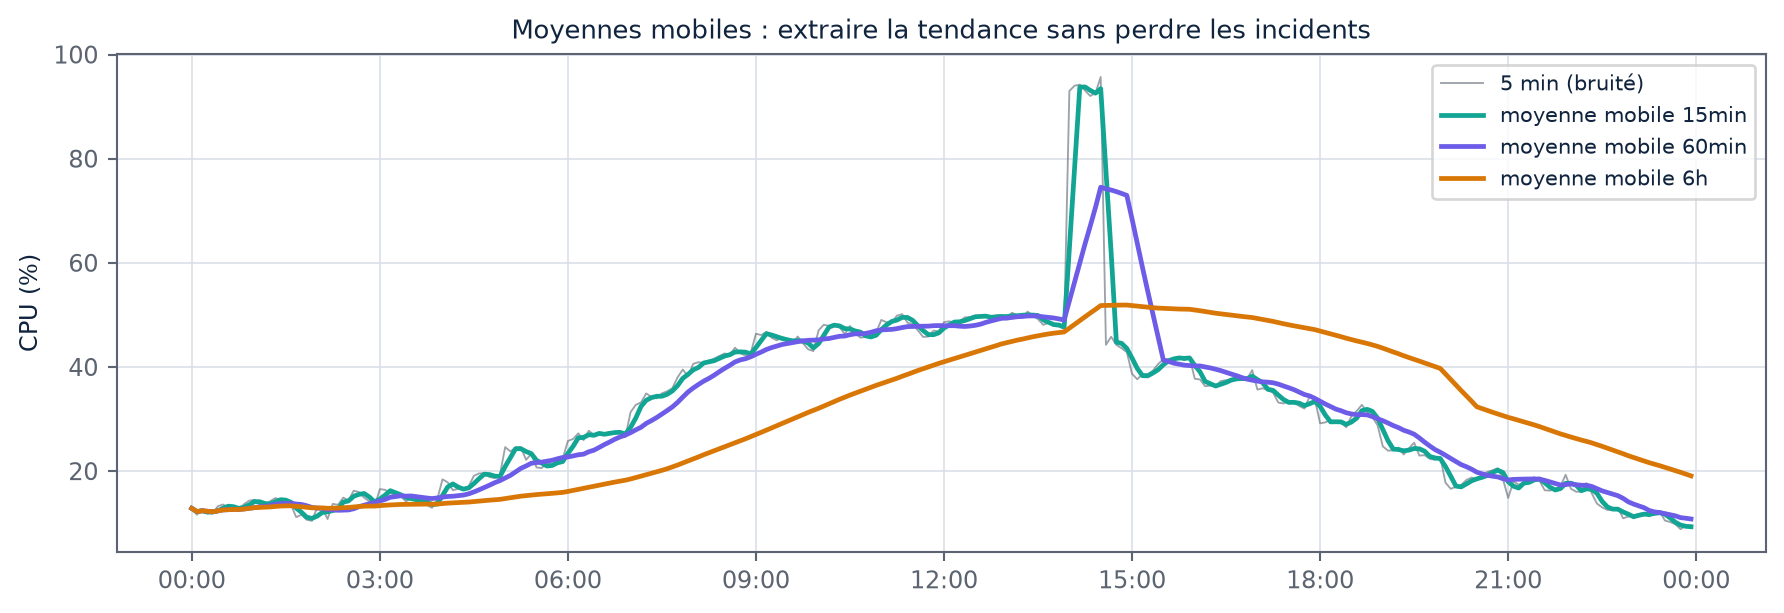
\includegraphics[width=0.94\textwidth]{f10_moyennes_mobiles.png}
\end{center}
\begin{columns}[t]
\begin{column}{0.5\textwidth}
\begin{ebox}[Lecture sur le jour de l'incident]
\begin{itemize}
\item 15 min : lisse le bruit, \textbf{garde} le pic de 14 h.
\item 60 min : donne la tendance, arrondit le pic.
\item 6 h : montre la saisonnalité jour/nuit, l'incident a disparu.
\end{itemize}
\end{ebox}
\end{column}
\begin{column}{0.46\textwidth}
\begin{kbox}[La règle de la fenêtre]
Choisir la fenêtre par rapport à ce qu'on veut prédire :
étiquette « incident $\le$ 30 min » $\Rightarrow$ signaux sur
\textbf{5 à 30 min}, jamais 6 h (l'information serait diluée).
\end{kbox}
\end{column}
\end{columns}
\end{frame}

\begin{frame}[fragile]{p99 par fenêtre : la variable qui voit la queue}
\begin{columns}[t]
\begin{column}{0.52\textwidth}
\begin{block}{Moyenne contre p99, par fenêtre de 10 min}
\begin{itemize}
\item La \textbf{moyenne} de latence est stable ($\approx$ 12 ms) --- même
pendant les prémices d'un incident.
\item Le \textbf{p99} par fenêtre explose \textbf{avant} que la moyenne ne
bouge : les requêtes lentes arrivent d'abord.
\item C'est pourquoi les SLO sont écrits en p99 (séance 1) --- et c'est
pourquoi nos features le seront aussi.
\end{itemize}
\end{block}
\begin{codebox}[En une ligne]
\begin{lstlisting}
f10 = (b.set_index("horodatage")
        .groupby("serveur")["latence_ms"]
        .resample("10min")
        .agg(lat_moy="mean", lat_p99=lambda s: s.quantile(0.99)))
\end{lstlisting}
\end{codebox}
\end{column}
\begin{column}{0.44\textwidth}
\begin{wbox}[Le piège du petit échantillon]
Sur une fenêtre de 10 min, il n'y a que \textbf{2 points} de métriques.
Le « p99 » de 2 points est presque le maximum --- c'est acceptable
(comme signal), mais il faut le \textbf{documenter} dans le dictionnaire
des variables : un p99 sur n=2 n'est pas un p99 statistique.
\end{wbox}
\begin{ebox}[Choix du pas du TP]
Métriques à 5 min $\Rightarrow$ fenêtre de \textbf{10 min} (2 points,
moyenne + max), étiquette regardant \textbf{30 min} en avant.
\end{ebox}
\end{column}
\end{columns}
\end{frame}

\begin{frame}[fragile]{Encodage cyclique : pourquoi 23 h et 0 h sont voisines}
\footnotesize%
\begin{center}
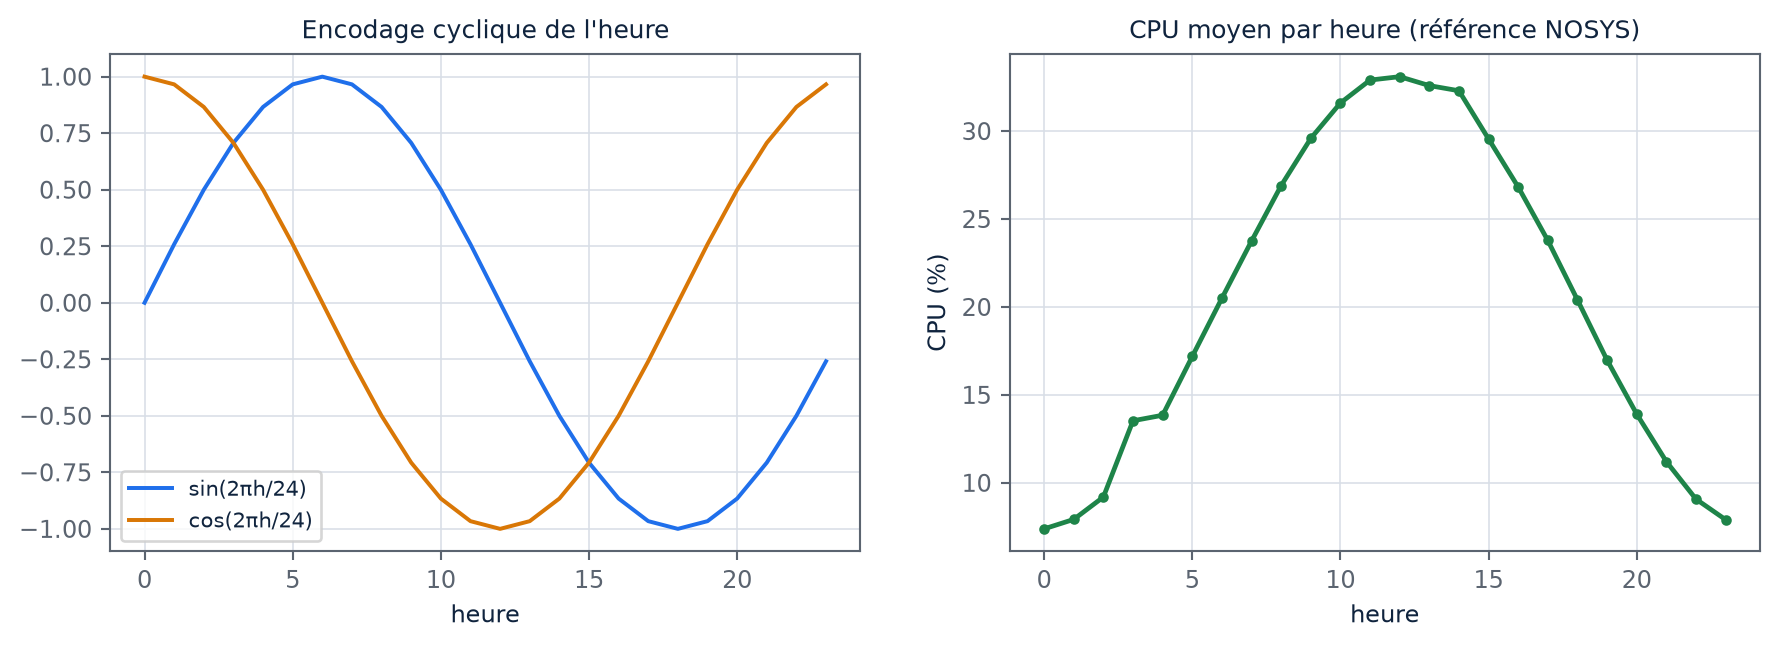
\includegraphics[width=0.80\textwidth]{f11_cyclique.png}
\end{center}
\begin{columns}[t]
\begin{column}{0.5\textwidth}
\begin{block}{Le problème de l'heure brute}
L'heure 23 et l'heure 0 sont \textbf{voisines} dans le réel
(1 h d'écart) mais \textbf{distantes de 23} dans la colonne brute.
Toute frontière cyclique (minuit, dimanche/lundi, décembre/janvier)
crée cette fausse discontinuité.
\end{block}
\begin{codebox}[La solution standard]
\begin{lstlisting}
h = b.index.hour
b["h_sin"] = np.sin(2*np.pi*h/24)
b["h_cos"] = np.cos(2*np.pi*h/24)
\end{lstlisting}
\end{codebox}
\end{column}
\begin{column}{0.46\textwidth}
\begin{kbox}[Pourquoi deux variables]
Un seul sinus replierait 6 h et 18 h sur la même valeur.
Le couple (sin, cos) place l'heure \textbf{sur un cercle} :
distance euclidienne = distance réelle entre heures.
Même traitement pour le \textbf{jour de semaine} (période 7)
et le \textbf{mois} (période 12).
\end{kbox}
\end{column}
\end{columns}
\end{frame}

\begin{frame}{La dérive de capteur : un défaut invisible aux seuils}
\footnotesize%
\begin{columns}[t]
\begin{column}{0.5\textwidth}
\begin{block}{Le cas srv-06}
Régression linéaire de la température sur le temps :
\begin{itemize}
\item pente mesurée : \textbf{+0,222 °C/jour} (fichier brut) ;
\item pente de référence (données propres) : $\approx$ 0.
\end{itemize}
Sur un mois : $+6{,}7$ °C --- sous aucun seuil, mais si la dérive
continue, la salle surchauffe \textbf{dans 2 mois}.
\end{block}
\begin{ebox}[Comment le détecter automatiquement]
Régression par fenêtre glissante (7 jours) : une pente
significativement $\ne$ 0 sur une métrique \emph{censée stationnaire}
= alerte de dérive. C'est un modèle \textbf{très simple qui remplace
un seuil impossible à écrire}.
\end{ebox}
\end{column}
\begin{column}{0.46\textwidth}
\begin{wbox}[Pourquoi les seuils ratent les dérives]
Un seuil alerte sur la \textbf{valeur absolue}. La dérive est un
problème de \textbf{tendance} : chaque valeur prise isolément est
normale, c'est leur \emph{enchaînement} qui ne l'est pas.
\end{wbox}
\begin{kbox}[Vocabulaire]
Ce test s'appelle \textbf{stationnarité} : une métrique de supervision
saine est stationnaire (moyenne et variance stables). On le formalisera
avec les séries temporelles (séance 4).
\end{kbox}
\end{column}
\end{columns}
\end{frame}

\begin{frame}{Standardiser : mettre toutes les échelles à égalité}
\footnotesize%
\begin{center}
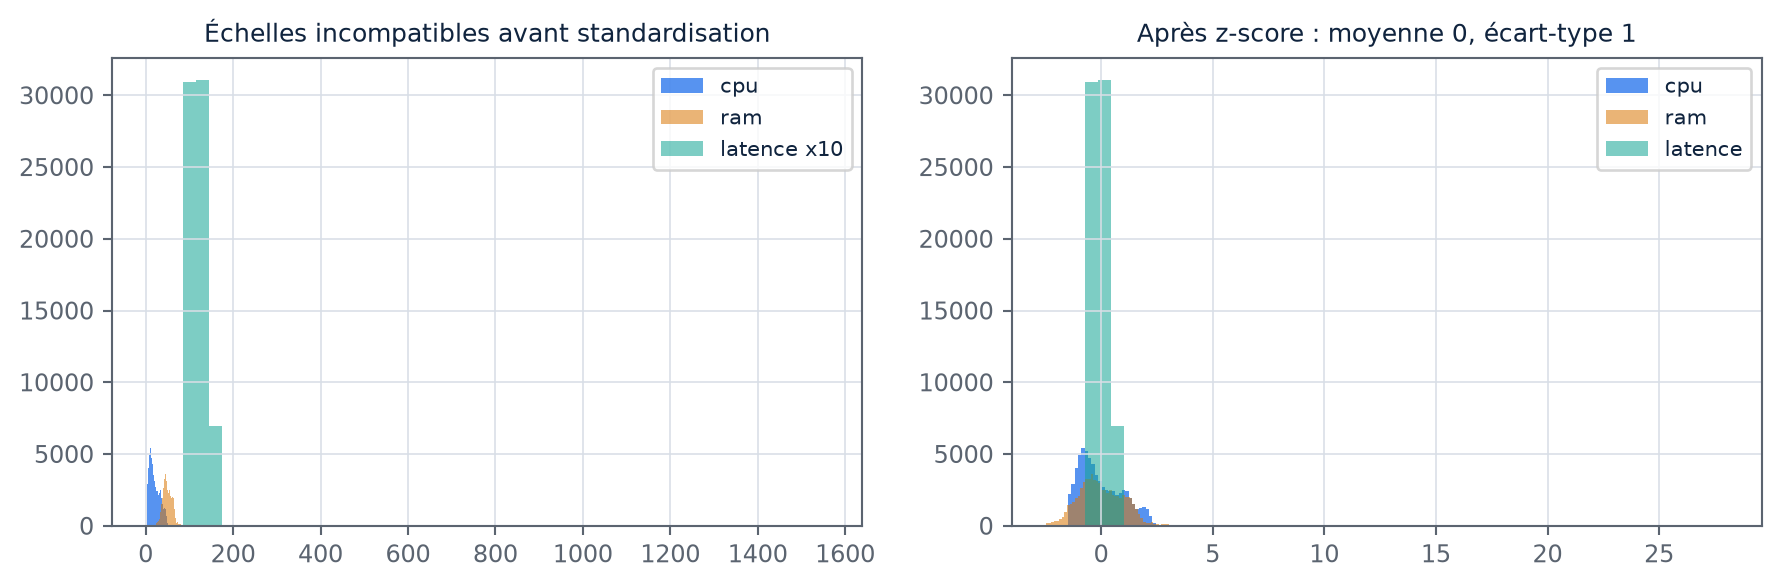
\includegraphics[width=0.94\textwidth]{f14_standardisation.png}
\end{center}
\begin{columns}[t]
\begin{column}{0.52\textwidth}
\begin{block}{Pourquoi c'est indispensable}
\begin{itemize}
\item CPU $\approx$ 20, RAM $\approx$ 50, latence $\approx$ 12 :
sans standardisation, un modèle à distances (k-NN, SVM) ou à
pénalité (ridge) est \textbf{dominé par la variable d'échelle la plus grande}.
\item $z = (x - \bar{x}) / \sigma$ : moyenne 0, écart-type 1.
\end{itemize}
\end{block}
\end{column}
\begin{column}{0.44\textwidth}
\begin{wbox}[Standardiser APRÈS le train/test split]
La moyenne et l'écart-type doivent être calculés \textbf{sur le train
seulement}, puis appliqués au test --- sinon on fait fuiter
l'information du futur. Avec les fenêtres temporelles de notre TP :
standardiser sur les 24 premiers jours, appliquer aux 6 derniers.
\end{wbox}
\end{column}
\end{columns}
\end{frame}

\begin{frame}{Quiz 3 --- signaux (5 min)}
\begin{qbox}[3 questions]
\begin{enumerate}
\item L'étiquette est « incident dans les 30 min ». La fenêtre de calcul
des signaux la mieux adaptée est :\\
(a) 6 h \quad (b) 24 h \quad (c) 5 à 30 min
\item Pourquoi encoder l'heure avec (sin, cos) plutôt qu'un nombre 0--23 ?\\
(a) c'est plus compact \quad (b) minuit sépare 23 h et 0 h alors qu'elles
sont voisines --- le cercle corrige \quad (c) les arbres l'exigent
\item La pente de température de srv-06 est +0,222 °C/jour. Le seuil
« alerte si T $>$ 45 °C » la détecte :\\
(a) immédiatement \quad (b) seulement quand la salle surchauffera ---
le seuil ne voit pas la \textbf{tendance} \quad (c) jamais
\end{enumerate}
\end{qbox}
\vspace{1mm}
\begin{solbox}[Réponses]
\textbf{1 : c} \quad \textbf{2 : b} \quad \textbf{3 : b} --- d'où la
régression glissante comme détecteur de dérive.
\end{solbox}
\end{frame}
